%! Author = fabian.sigfridsson
%! Date = 2023-04-19

\documentclass[11p]{article}
% Packages
\usepackage{amsmath}
\usepackage{graphicx}
\usepackage[swedish]{babel}
\usepackage[
    backend=biber,
    style=authoryear-ibid,
    sorting=ynt
]{biblatex}
\usepackage[utf8]{inputenc}
\usepackage[T1]{fontenc}
\usepackage{hyperref}
%Källor
% \addbibresource{mall.bib}
\graphicspath{ {images/} }

\def\name{Fabian Sigfridsson}
\def\email{fabian.sigfridsson@elev.ga.ntig.se}

\title{Labbrapport \\ \small Fysik 1}
\author{\name}
\date{\today}

\begin{document}

%    1
%    0,03V
%    0,0003A
%    0,03/0,0003 = 100 ohm
%    2
%    0,015V
%    0,0003A
%    0,015/0,0003 = 50 ohm
%    3
%    0,03V
%    0,00015A
%    0,03/0,0003 = 100 ohm

    \begin{titlepage}
        \begin{center}
            \vspace*{1cm}

            \Huge
            \textbf{Laboration 5}

            \vspace{0.5cm}
            \LARGE
            Ellära

            \vspace{1.5cm}

            \textbf{\name}

            \vfill


            Fysik 1

            \vspace{0.8cm}

            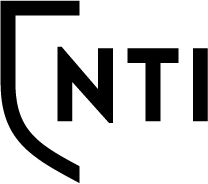
\includegraphics[width=0.4\textwidth]{images/NTI_Gymnasiet_Symbol_print_svart}

            \Large
            Teknikprogrammet\\
            NTI Gymnasiet\\
            Umeå\\
            \today

        \end{center}
    \end{titlepage}
    \section{Syfte och frågeställning}
    \section{Material}
        \begin{itemize}
            \item 1 Batteri
            \item 1 Multimeter
            \item 4 Kablar
            \item 2 Resistorer
            \item 6 Krokodilklämmor
            \item 3 Kopplingsplintar
        \end{itemize}
    \section{Del 1}
    \subsection{Metod}
        \begin{enumerate}
            \item Vi kopplade batteriet till motståndet
            \item Vi mätte spänningen över motståndet
            \begin{figure}[!h]
                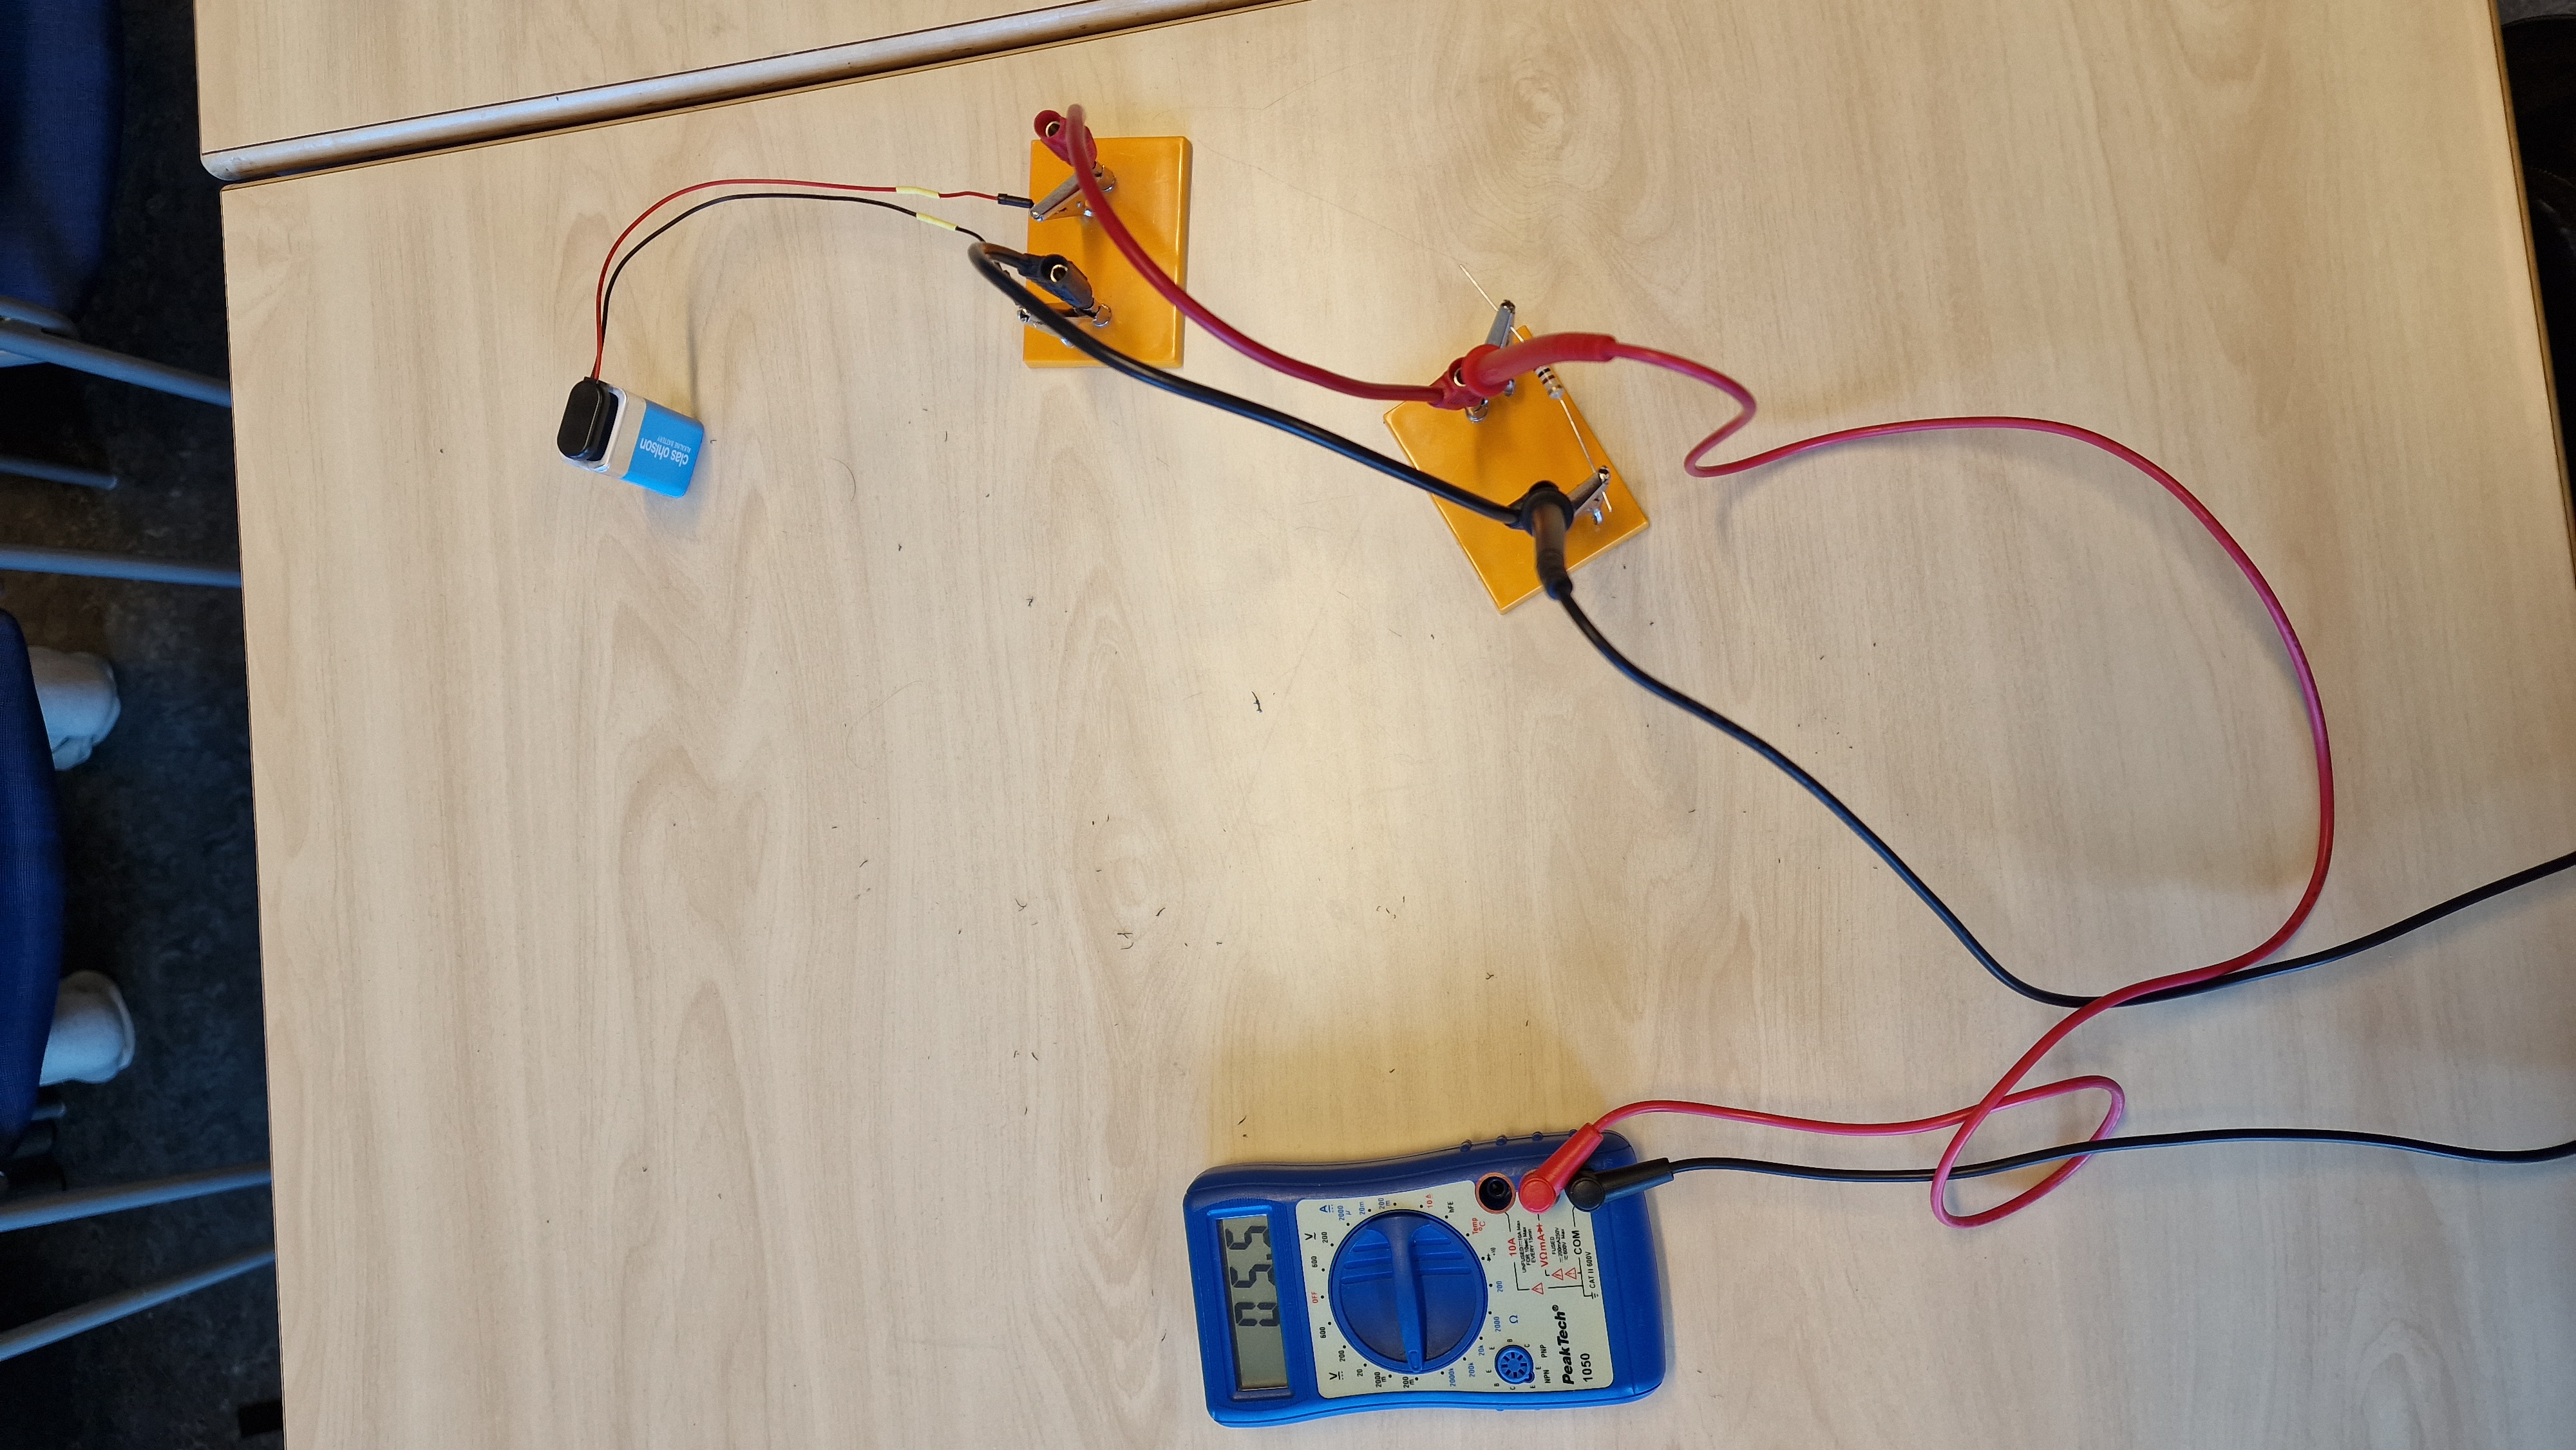
\includegraphics[width=0.8\textwidth]{images/enkelVolt}
                \caption{Volt över motståndet}
                \label{fig:eV}
            \end{figure}
            \item Vi mätte strömmen i kretsen
            \item Vi mätte spänningen över kretsen
        \end{enumerate}
    \newpage
    \subsection{Resultat}
        Strömmen genom motståndet uppmättes till 0,03V.
    \linebreak
        Spänningen över motståndet uppmättes till 0,0003 A.

    \subsection{Analys}
        \begin{equation}
            R=\frac{U}{I}
            \label{eq:ohms-lag}
        \end{equation}
        Vi kan då se att enligt Ohms lag \ref{eq:ohms-lag} så blir
        motståndet i resistorn \frac{0,03V}{0,0003A} = 100\Omega

    \section{Del 2}
    \subsection{Metod}
        \begin{enumerate}
            \item
        \end{enumerate}
    \subsection{Resultat}

    \subsection{Analys}

    \section{Del 3}
    \subsection{Metod}
    \subsection{Resultat}
    \subsection{Analys}
    \section{Diskussion}
\end{document}